
\documentclass[a4paper,11pt]{article}

\usepackage{graphicx}
\usepackage{enumerate}
\usepackage{epstopdf}
\usepackage{alltt}
\usepackage[margin=1.4in,vmargin=1.3in]{geometry}
\abovecaptionskip 0in
\belowcaptionskip 0.06in
% \usepackage{titling}
\newcommand{\subtitle}[1]{
  \posttitle{
    \par\end{center}
    \begin{center}\large#1\end{center}
    \vskip0.5em}
}

\title{ Acoustic Modem Project:}
% \subtitle{Audio Playback, recording and analysis}
\author{Frederic Mes, Wim Marynissen}
 \date{\today}


\begin{document}
\maketitle
\section{Session 1}
\subsection{Exercise 1: Audio playback/recording}
Done.

%\subsection{Another subtitle}

\subsection{Exercise 2: Time-frequency analysis of recorded signals}
\begin{alltt}
	2.	There's some noise besides the 400Hz frequency.
	
	3.	The DFT size determines the time interval of which a spectrum is calculated.
		(+ opgeschreven uitleg)
		
	4.	There are other frequencies present. These are harmonic frequencies, they are
	multiples of the original frequency.
	
	5.	In the spectrogram of the transmitted signal, there's a DC component. But in
	the recorded signal this DC component has faded. 
	
	6.	Clipping amplifies some of the harmonic frequencies. This could be harmful
	for the acoustic modem for harmonic signals could interfere with the correct
	signal. (?)
	
	8.	?
	
	9. It shows which frequency range is let trough by the channel.
	
	10. It doesn't change over time. This is relevant because we want a
	time-invariant system.
	
	11. There's more background noise and a weaker signal. (?)
\end{alltt}

\subsection{Exercise 3: Time-frequency analysis of recorded signals}
\begin{alltt}
1. Schatting dmv ruis: 500-6500 Hz,

4. The maximum data transfer rate for error-free transmission, in bits per
second.
\end{alltt}
\section{Session 2}
\subsection{Exercise 2-1}
\begin{alltt}
1.	

2.	The estimated IR contains approx. 100 samples

3.	The IR length would be bigger

4.	

5.	They do look more or less the same.
	Explenation: white noise has a constant PSD so the channel transferfunction is
	multiplied with a constant.

\end{alltt}
\subsection{Exercise 2-2}
\begin{alltt}
1.



2.	

3.

4.

5.

6.
\end{alltt}
\clearpage
\subsection{Exercise 2-3}
\begin{alltt}
1.	No, IR2.M always results in more or less thesame graph:
	\begin{figure}[h]
	  		\begin{center}
				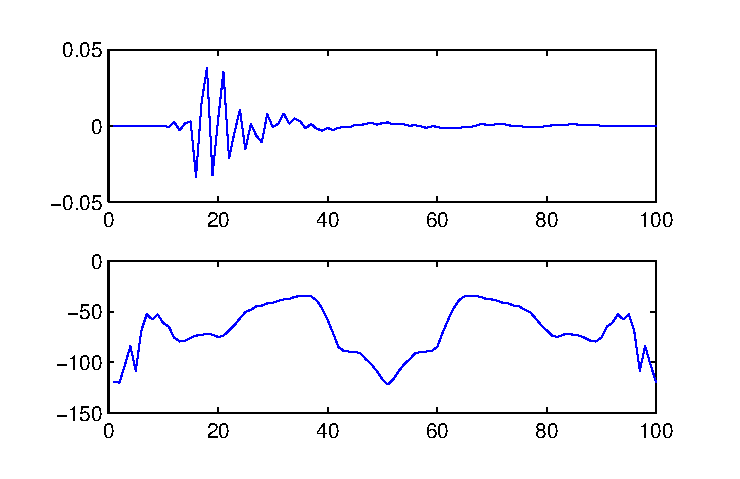
\includegraphics[width=0.65\textwidth]{Sessie2/IR2.eps}
			\end{center}
			\label{benadering}
  	\end{figure}


4. Yes, the shape of the frequency responses changes over different experiments.
	\begin{figure}[H]
	  		\begin{center}
				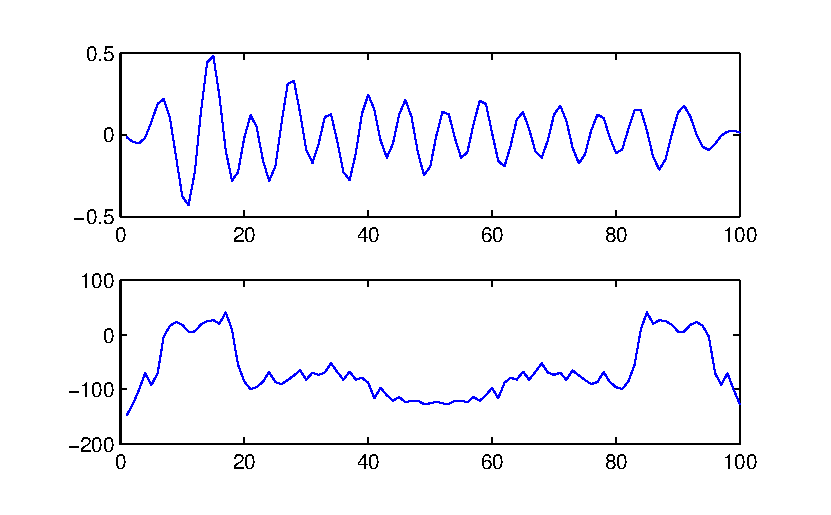
\includegraphics[width=0.65\textwidth]{Sessie2/IRbs1.eps}
			\end{center}
			\label{benadering}
  	\end{figure}
  
  	
  	\begin{figure}[H]
	  		\begin{center}
				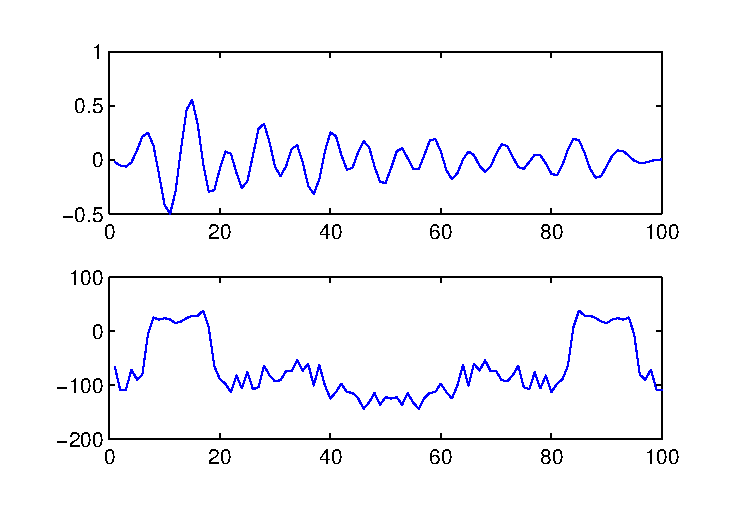
\includegraphics[width=0.65\textwidth]{Sessie2/IRbs2.eps}
			\end{center}
			\label{benadering}
  	\end{figure}
  
  	\begin{figure}[H]
	  		\begin{center}
				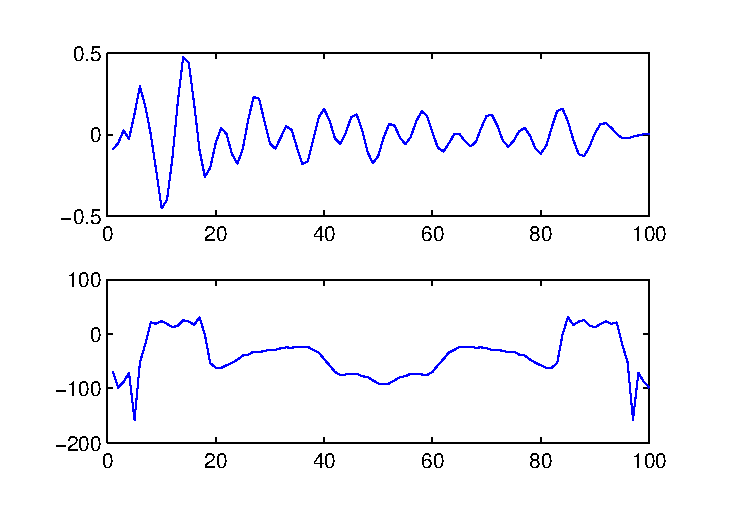
\includegraphics[width=0.65\textwidth]{Sessie2/IRbs3.eps}
			\end{center}
			\label{benadering}
  	\end{figure}


\end{alltt}
\end{document}
